\documentclass[11pt]{article}
\usepackage{uarial}
\renewcommand{\familydefault}{\sfdefault}
\usepackage{fullpage}
\usepackage{setspace}
\usepackage{parskip}
\usepackage{titlesec}
\usepackage[section]{placeins}
\usepackage{xcolor}
\usepackage{breakcites}
\usepackage{lineno}
\usepackage{hyphenat}
\usepackage[labelfont=bf, labelsep=period]{caption}
\usepackage{times}
\usepackage{etoolbox}
\usepackage[numbers]{natbib}
\usepackage{graphicx}
\usepackage[space]{grffile}
\usepackage{latexsym}
\usepackage{textcomp}
\usepackage{longtable}
\usepackage{tabulary}
\usepackage{booktabs,array,multirow}
\usepackage{amsfonts,amsmath,amssymb}
\usepackage{enumitem}
\usepackage{varwidth}
\usepackage{microtype}
\usepackage{subfig}
\providecommand\citet{\cite}
\providecommand\citep{\cite}
\providecommand\citealt{\cite}
\usepackage[utf8]{inputenc}
\usepackage[T1]{fontenc}
\usepackage[english]{babel}
\usepackage[colorlinks = true,
            linkcolor = blue,
            urlcolor  = blue,
            citecolor = blue,
            anchorcolor = blue]{hyperref}
\begin{document}

\author{Adam Kimbler}

\begin{titlepage}
    \begin{center}
        \textbf{Neurobiological Contributions of Pubertal Development, Top-down control
            of Emotional Arousal, and Reward Processing on Mnemonic Performance}

        \vspace{0.8cm}
        PROPOSAL FOR DISSERTATION\\
        DOCTOR OF PHILOSOPHY IN COGNITIVE NEUROSCIENCE, PSYCHOLOGY\\
        COLLEGE OF ARTS, SCIENCES AND EDUCATION\\
        \vspace{0.8cm}
        Adam Kimbler\\
        DEPARTMENT OF PSYCHOLOGY, FLORIDA INTERNATIONAL UNIVERSITY, MIAMI, FL, 33199
        08/11/2022
    \end{center}
    \vspace*{\fill}
    I propose to Major Professor (Aaron T. Mattfeld, PhD) and Committee Members
    (Timothy Allen, PhD, Dana McMakin, PhD, and Matthew DeGennaro, PhD), a
    functional magnetic resonance imaging and behavior study to be conducted in
    fulfillment of requirements for Doctor of Philosophy in Psychology with an
    emphasis in Cognitive Neuroscience.
\end{titlepage}
\clearpage

\section*{Background and Significance}

The hippocampus is a structure that plays a crucial role in forming and retrieving
episodic memories, which are memories for the what, when, and where of an event. One
possible explanation for how episodic memories are formed and stored is through the
processes of pattern separation and completion, which characterizes how a new event may
be stored orthogonally to (pattern separation) or together with (pattern completion)
previous contextual information \citep{yassa_ability_2011}. The hippocampus, with its
multiple distinct subregions, appears particularly suited for the operations of pattern
separation and completion. The dentate gyrus (DG), with its strong excitatory granule
cells and sparse connections is thought to play an important role in pattern separation
\citep{treves_mammalian_dentate_2008,
mcnaughton_hippocampal_1987,blackstad_distribution_1970,swanson_autoradiographic_1978},
while the CA1
\citep{burke_shared_function_2018,bakker_pattern_2008,rolls_quantitative_2013,
bittner_conjunctive_2015} and CA3
\citep{Insausti_Amaral_2008,trevino_excitationinhibition_2011} receive multiple sources
of input and likely play important roles in pattern completion. These processes are
often assessed in humans by using mnemonic similarity tasks (MST), that examine what
are thought to be behavioral correlates of pattern separation and completion: mnemonic
discrimination and generalization. \par

The hippocampus also shares connectivity with numerous systems in the brain including
those for reward \citep{lisman_neohebbian_2011,kempadoo_dopamine_2016} and arousal
\citep{yang_bla_2016,yang_bla_2017}. Despite these known patterns of regional
connectivity, little work has been done across the literature demonstrating how these
connections impact mnemonic generalization in humans. 

\section*{Research Objectives and Questions}
In this dissertation, I outline two objectives to investigate how pubertal
development and reward processing contribute to
mnemonic performance.\par
\textbf{Aim 1: }\textit{Characterize changes in memory discrimination/generalization for
    valenced information related to medial temporal lobe development.} \par
\textbf{Aim 2: }\textit{Examine how reward and loss relate to mnemonic
    discrimination and generalization.} \par

\section*{Experimental Design, Hypotheses, and Preliminary Data}

\subsection*{AIM 1: Characterize changes in memory discrimination/generalization for
    valenced information related to medial temporal lobe development.}
Memory increases in specificity, driven by maturation of key neurobiological substrate
taking root around the onset of puberty and continuing into adolescence
\citep{Lavenex2007, Lee2014,Daugherty2017,Keresztes2018}. Whether these
specificity-supporting neurobiological mechanisms are similarly employed across
different stimulus valences (e.g.,\ emotional versus neutral) remains unknown. Around
the same developmental window, the prevalence of anxiety disorders increases
\citep{Beesdo2009}. Together, understanding how developmental differences in memory
specificity interact with emotional salience of stimuli may provide important insight
into our understanding of negative overgeneralization, a characteristic symptom of
anxiety where individuals generalize negative associations to similar events
\citep{Lissek2014}. In pursuit of Aim 2, we seek to understand the relation between
cross-sectional indices of neurobiological maturation around the onset of adolescence
and measures of behavioral discrimination and generalization to stimuli with emotional
valence. Data from a two-session magnetic resonance imaging (MRI) study in which
participants completed the study and test sessions of an emotional mnemonic similarity
task with a twelve-hour delay between sessions was analyzed. In this analysis, I sought
to examine how the level of pubertal maturity in the hippocampus predicted mnemonic
generalization and completion for negative and neutral images. To answer this question,
I examined how emotional valence and hippocampal pubertal maturation interacted to
predict lure discrimination (LDI) and generalization (LGI) performance. I expected to
observe an increase in neutral lure discrimination performance (LDI) with increasing
hippocampal pubertal maturity index (PMI), with neutral lure generalization (LGI)
remaining relatively stable. We also expected the relationship between negative LDI and
LGI to differ for negative stimuli. We also expect that any relationships between PMI
and mnemonic performance will be localized to the hippocampal formation (HF), rather
than other MTL regions such as the rhinal cortices or amygdala (AMY).

\subsubsection*{Regional Volumetric and Connective Pubertal Maturity Index: PMI}
To calculate regional maturity scores partial least squares correlation (PLSC) was
conducted to produce regional maturity for the HF (DG/CA2/CA3/CA4, CA1, subiculum,
posterolateral and anteromedial entorhinal cortices), rhinal (RHI) cortices (perirhinal
cortex and parahippocampal cortex), and amygdala (AMY) (resulting k-means clusters
determined by probabilistic tractography) according to an approach first outlined by
~\cite{keresztes_adaptive_2017}. Due to the nature of our sample, and the strong effects
of pubertal status on development within our age range, the Pubertal Development Scale
(PDS) was used in lieu of age in construction of maturity scores. The PDS was scored so
that the value obtained roughly equivocated Tanner staging
\citep{shirtcliff_pubertal_2009}. A correlation matrix was produced by PDS-Shirtcliff
and volumetric measures for each ROI\@. The resultant matrix was then decomposed via
singular value decomposition (SVD). Resultant weights for each ROI were
then multiplied by each subject's vector of ROI volumes to produce a singular regional
maturity score. This process was completed for the HF, RHI and AMY to produce
Hippocampal, Amygdala, and Rhinal PMI, respectively. This PLSC analysis was conducted
using NumPy (1.19.4) \citep{harris_numpy_2020} in Python 3.8.3.
PLSC was also used to compute connectivity maturity metrics between regions. A
correlation matrix was constructed using total PDS score and the median number of random
walks between the seed and target regions. This matrix was decomposed via SVD and the
resultant weights were multiplied by the median connection strength to produce a
connectivity maturity score. This was conducted for the following connections:
Amygdala to HF, HF to Rhinal Cortices, and HF to mPFC\@. These formed the basis of our
Amy-HF connectivity, HF-RHI connectivity, and HF-mPFC
connectivity PMI scores respectively.

\subsubsection*{Emotional Mnemonic Similarity Task: eMST.} Participants took part in an
emotional similarity task that consisted of an incidental encoding session and a
followup test session approximately 12 hours later. During the incidental encoding
session, participants were asked to rate scene images as negative, neutral or positively
valenced. Participants returned 12 hours later and completed a recognition memory task
that asked them to rate images as old (they saw during encoding) or new (they did not
see the images during encoding), with the caveat that some of these images would be
similar, but not the same as images during encoding. Performance on these similar
images, referred to as lures, was used to calculate LDI and LGI performance. For more
information, see~\cite{mcmakin_negative_2021} and \hyperref[fig:1]{Fig.\ 1A}. \par

\subsubsection*{Data Analysis.} Structural magnetic resonance imaging (sMRI) and
diffusion magnetic resonance imaging (dMRI) were used along with clinical measures of
pubertal maturity to produced volumetric and
connective estimates of PMI to address the following research questions:
\begin{enumerate}
    \item Determine if increasing volumetric PMI in the HF is associated with increased
          lure discrimination performance for neutral images, and if this relationship
          holds for negative images; \textit{examine the results of two mixed effects
              linear models predicting LGI and LDI, with age, gender, image valence, HF
              volumetric PMI, and image valence X HF volumetric PMI as predictors.}
          \textbf{Prediction}: The interaction between image valence X HF volumetric PMI
          will be a significant predictor of LGI and LDI performance
    \item Determine if this relationship between volumetric PMI is unique to the
          hippocampus; \textit{examine the results of several mixed effects linear
              models predicting LGI and LDI, with age, gender, image valence, RHI/AMY
              volumetric PMI, and image valence X RHI/AMY volumetric PMI as predictors.}
          \textbf{Prediction}: The interaction between image valence X RHI/AMY
          volumetric PMI will not be a significant predictor of LGI and LDI performance.
    \item Explore if similar interactions occur when PMI is examined based on
          diffusion-based regional connectivity (AMY to HF, HF to RHI, HF to mPFC),
          rather than volumetric PMI\@; \textit{examine the results of several mixed
              effects linear models predicting LGI and LDI, with age, gender, image
              valence, AMY to HF/HF to RHI/HF to mPFC connectivity PMI, and image
              valence X AMY to HF/HF to RHI/HF to mPFC volumetric PMI as predictors.} 
              \textbf{Prediction}: There will be an interaction between image X regional
              connectivity PMI for the examined connections (AMY to HF, HF to RHI, HF to
              mPFC)
\end{enumerate}

\subsubsection*{Results.}
\begin{enumerate}
    \item As predicted, we identified a significant interaction between HF volumetric
          PMI and stimulus valence predicting LDI and LGI\@.
          (\hyperref[fig:1]{Fig.\ 1B}). We observed that HF volumetric PMI was
          associated with greater discrimination of neutral images, and limited or
          minimally reduced discrimination of negative images. We found enhanced
          generalization of negative images associated with greater HF volumetric PMI,
          while neutral generalization remained steady or decreased slightly as a
          function of HF volumetric PMI (\hyperref[fig:1]{Fig.\ 1B}).
    \item Divergent patterns were not observed in discrimination (LDI) across PMI and
          image valence in the rhinal cortices or the amygdala. Rhinal volumetric PMI
          significantly interacted with stimulus valence when predicting LGI, while
          amygdala maturity did not. As rhinal maturity increased, LGI decreased for
          negative images, and increased for neutral images.
    \item We did not identify an interaction between AMY-HF connectivity PMI and
          stimulus valence predicting LDI, or LGI\@. We did not identify an interaction
          between HF-RHI connectivity PMI and stimulus valence predicting LDI or LGI\@.
          When comparing discrimination across image valence (negative and neutral) and
          our HF-mPFC connectivity PMI we observed a trend towards differential
          discrimination following corrections for multiple comparisons. Negative image
          discrimination was reduced with elevated HF-mPFC connectivity PMI, while
          greater neutral image discrimination was evident with greater HF-mPFC
          connectivity PMI\@. Generalization exhibited a significant relationship with
          valence in the opposite pattern, with greater HF-mPFC connectivity PMI
          associated with greater negative image generalization, and reduced neutral
          image generalization.
\end{enumerate}
\begin{figure}%
    \centering
    \subfloat[\centering{Task Design}]{
        {\includegraphics[width=7cm]{figures/aim_1_task.png}}}%
    \qquad
    \subfloat[\centering{Hippocampal Subfields and Results}]{
        {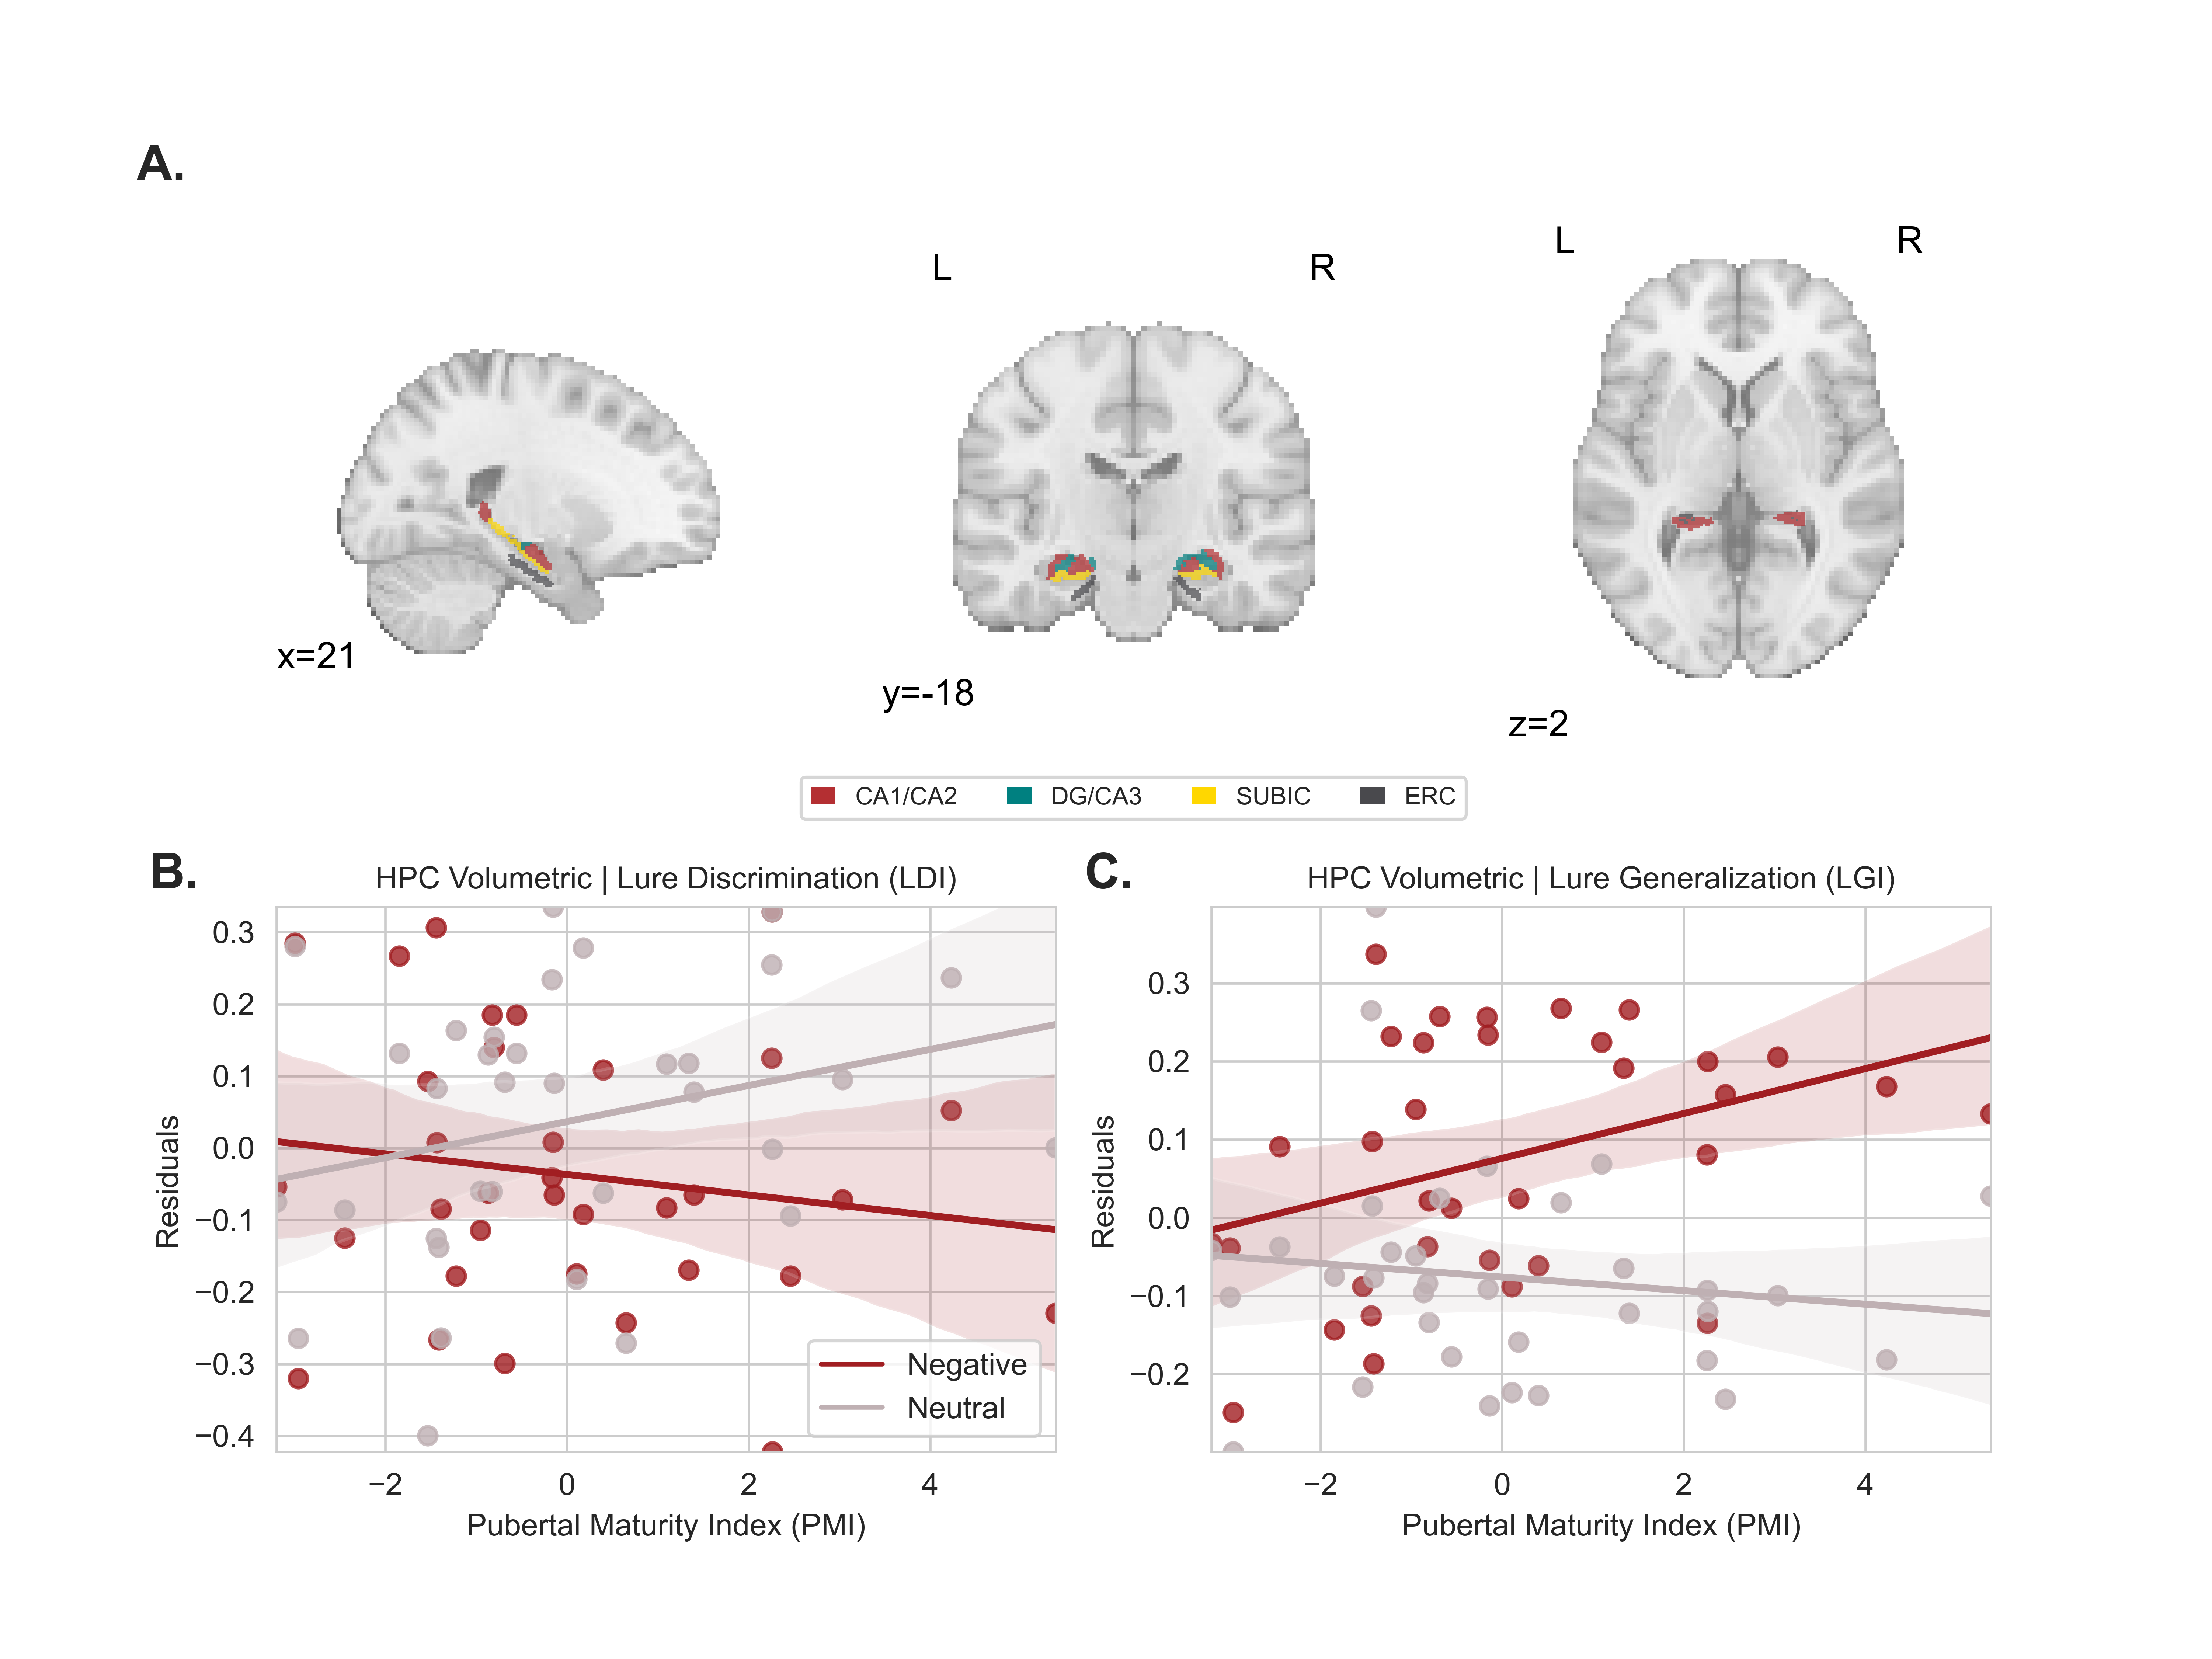
\includegraphics[width=7cm]{figures/aim_1_results.png}}}%
    \caption{Aim 1 Task Progression}%
    \label{fig:1}%
\end{figure}

Aim 1 is complete, and the resulting manuscript is currently under review at Learning
\& Memory as of Summer 2022
\subsection*{AIM 2: Examine how avoided loss and unexpected loss impact mnemonic
    discrimination and generalization using a performance-based behavioral paradigm.}
Manipulating dopaminergic reward-based pathways has long been the domain of
classical conditioning paradigms, which have consistently shown VTA neurons responding
to cues of reward anticipation \citep{fiorillo_discrete_2003}. DA from the VTA in
responses to reward has been shown to produce long-term potentiation based protein
synthesis in the CA1 subfield of the hippocampus, providing more evidence that DA is
potentially biasing the system toward pattern completion \citep{huang_lateltp_1995}. In
human fMRI research regional co-activation between the VTA, ventral striatum, and
hippocampus has been shown to predict superior memory performance
\citep{adcock_reward-motivated_2006}. This finding, however, comes with the caveat that
memory specificity was not tested, and this improved memory performance may come at the
cost of a more generalized memory representation. Other studies have found that these
same regions are active during reward and loss learning preceding improved memory
performance during recognition memory tasks \citep{shigemune_remembering_2014}. DA
impacts memory performance by promoting pattern completion processes in the CA1 region
of the hippocampus \citep{kempadoo_dopamine_2016}, with disruptions in DA signaling
leading to poorer performance when given degraded memory cues \citep{li_balanced_2010}.
Thus, modulation of DA in the hippocampus through reward based manipulations appears to
bias the system toward pattern completion. \par

Within functional neuroimaging paradigms, reward responses often take the form of
changes in signal within the ventral striatum. This ``reward prediction error'' (RPE)
signal results in increased signal in the ventral striatum following a trial that was
successfully rewarded \citep{schultz_reward_1997,daw_rewardprediction_2011}. Models
examining RPE have found that rather than total information influencing received reward,
an event is rewarding based on the gap between expected and received reward
\citep{marvin_curiosity_2016}. Additionally, these hippocampal signal also changes in
response to RPEs \citep{davidow_upside_2016}. These signals are likely due to the
excitation induced by DA neurons following a reward. While these paradigms often examine
RPE in response to reward and loss within a task, very few studies examine the effect of
averted losses (trials that were expected to be a loss, but were avoided), which should
have a similar impact to reward. \par

For Aim 2, I will examine how loss and reward impact memory performance, expanding
the current literature by examining the impact of averted loss and gain, and using a
novel performance-based reward paradigm. Participants completed a performance-based loss
aversion task consisting of two sessions, Study and Test, with the study session taking
place in an MRI scanner. In this experiment, I sought to determine how loss and reward,
as well as averted loss and reward influence memory performance. I expect that trials
that were rewarded would be better recognized, and that trials where loss was averted
would show similar memory performance. I also expect that lure generalization will be
higher for these rewarded or loss-averted trials compared to neutral trials.

\subsubsection*{Loss Aversion Assessment Task: LAVA.}
The task consisted of two sessions, an incidental encoding session in the MRI scanner
and a behavioral-only recognition memory test 24 hours later. During the encoding
session participants were shown object images and were instructed to endorse whether the
object was more typically found indoors or outdoors. Each object image was accompanied
by a cue in the form of a box in one of three colors indicating whether the participant
would gain (green; 72 images), lose (red; 72 images), or maintain (gray; 72 images)
arbitrary points on the given trial. Participants were instructed that they would be
given points for each correct answer on gain trials, would lose a point for each
incorrect answer on loss trials, and would neither gain nor lose on maintain trials.
Importantly, they were informed that scoring 25 or more points on the task would reward
them with an additional twenty dollars. For each encoding trial, the cue + stimulus pair
was presented for 2000ms. This was followed by an interstimulus interval (ISI) of
2000--6000ms. Then, a Go! Prompt was given for 500ms indicating the participant should
give their indoor or outdoor rating. This response window was followed by another
2000--6000ms ISI, then a Feedback window showing whether the response was correct or
incorrect and how many points were gained or lost on the trial. After completing the
task, participants returned 24 hours later for a surprise recognition memory task.
During the recognition memory task, participants were shown object images that were
either presented during encoding (targets; 108 images), were similar to those during
encoding (lures; 108 images), or were completely new (foils; 108 images) and were asked
to rate the images as Old or New. This task was self-paced.

\subsubsection*{Neuroimaging data collection and preprocessing.}
Magnetic resonance imaging data was collected on a Siemens Magnetom Prisma 3T scanner
with a 32-channel head coil at the Center for Imaging Science at Florida International
University (Miami, FL). Functional data was obtained using T2*-sensitive gradient echo
pulse  sequence (66 interleaved axial slices, slice thickness = 2.0 mm, TR = 1760 ms,
TE = 35 ms, flip angle = 52\textdegree, field of view (FOV) = 200 mm, voxel size =
\(2.0 \times 2.0 \times 2.0 mm^2\)). Four hundred and seventy-seven whole-brain images 
were collected per experimental run. To ensure stabilization of magnetic resonance
signal, acquisition of data began after the fourth volume. For purposes of
coregistration and registration, high-resolution three-dimensional
magnetization-prepared rapid gradient echo sequence collected (MP-RAGE\@: 176 axial
slices, slice thickness = 1.0 mm, TR = 2500 ms, TE = 2.9 ms, flip angle = 8\textdegree,
FOV = 256 mm, voxel size = \(1.0 \times 1.0 \times 1.0 mm^3\)). Functional Neuroimaging
data are preprocessed using standard methods using fMRIPrep
\citep{esteban_fmriprep_2022}.

\begin{figure}%
    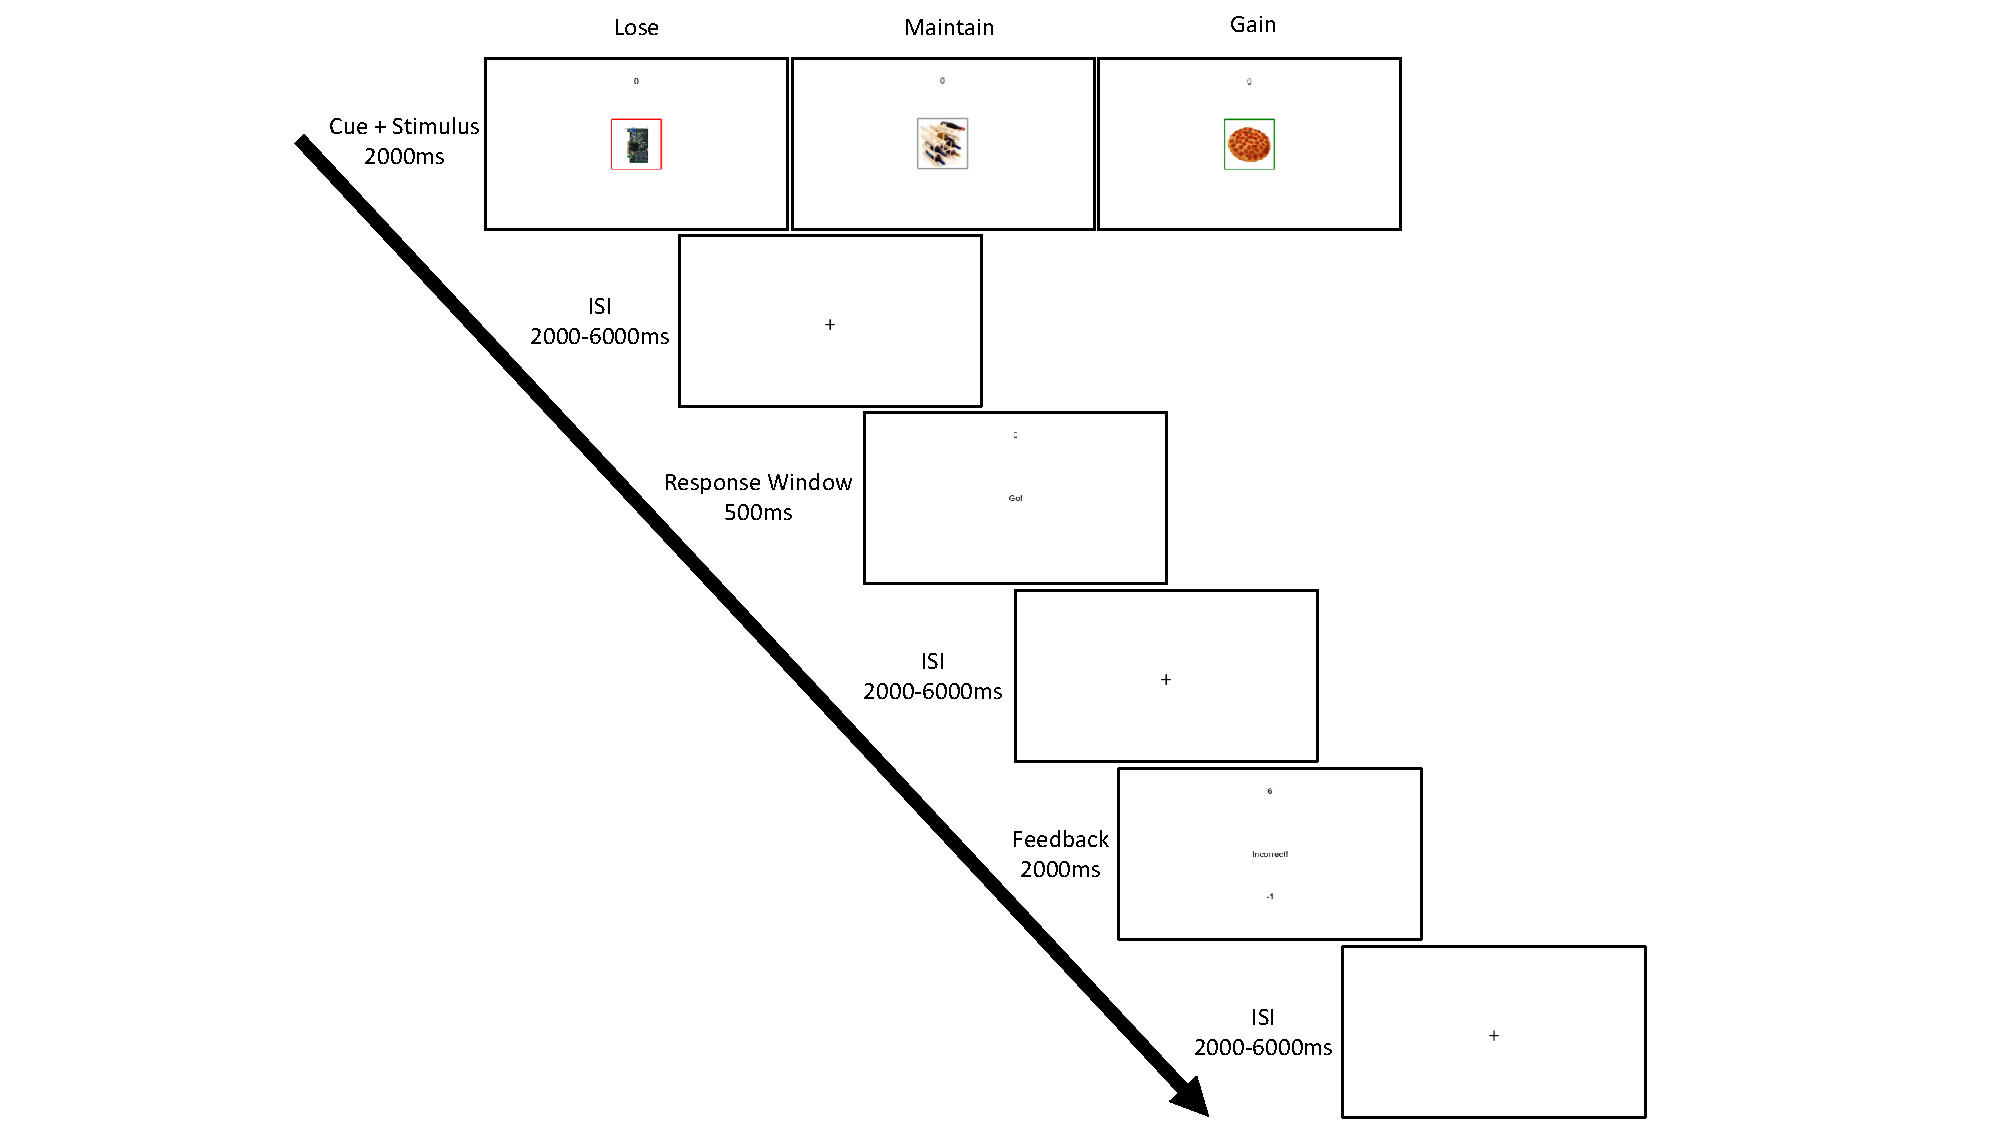
\includegraphics[width=14cm]{figures/aim_2_task.pdf}%
    \caption{Hippocampal Pubertal Maturity is associated with increased discrimination
        of neutral images and increased generalization of negative images}%
    \label{fig:2}%
\end{figure}
\subsubsection*{Data Analysis.} Functional magnetic resonance imaging (fMRI) using
anatomical regions of interest (ROI) will be conducted to address the following research
questions
\begin{enumerate}
    \item Determine the impact of reward and averted loss on subsequent memory
          performance for targets and lures; \textit{examine the results of three mixed
              effects linear models predicting LGI, LDI, and recognition memory
              performance with age, gender, and trial-type as predictors.}
            \textbf{Prediction}: Trial-type will be a significant predictor of LGI, LDI, and
            recognition memory performance. Further, I expect post-hoc tests to reveal
            that this difference is driven by higher recognition memory and LGI for
            rewarded and loss-averted trials compared to maintain trials. These findings
            will provide evidence that loss-averted trials have similar impact on memory
            as loss and reward themselves.
    \item ROI analysis examining hippocampus and ventral tegmental area (VTA) for reward
          and loss-averted trials; \textit{differences in fMRI based activation in the
              VTA and HPC ROI defined using FreeSurfer parcellation and segmentation
              (aparc+aseg) \citep{dale:99} between reward versus maintain trials and
              loss-averted versus maintain
              trials.}
            \textbf{Prediction}: Higher levels of activation in the VTA for reward and loss-averted
            trials relative to maintain trials. This provides evidence that VTA activation
            at time of encoding differs depending on type of trial, and potentially
            impacts subsequent memory encoding.
\end{enumerate}

\clearpage
\selectlanguage{english}
\bibliographystyle{ieeetr}
\bibliography{diss_proposal.bib}{}
\end{document}